\chapter{Fast One-Ring Smoothing: Mathematical Grounding}
\label{ch4}
In this one, and the next two chapters, we present an updated version of \Fors{t}, based on the ideas initially proposed by H. Mara and S. Krömker at the EUROGRAPHICS Workshop on Graphics and Cultural Heritage (2017) ~\cite[s.~3.2]{Mara17}. Since publication, further research has been conducted by the authors, and it was determined that improvments to the weighting methods were possible, therefore, modifications to the algorithm were implemented directly within the GigaMesh \todoCitation{GigaMesh} framework. This chapter presents the mathematical grounding for the as-yet-unpublished version of \fors{t}, as it exists now in GigaMesh, with more accurate weighting methods based on the interpolation and extrapolation of function values to the center of gravity of each circular sector comprising the geodesic disc centered upon each point in a triangle mesh of \tdd{}.

The procedure for designing any convolutional filter must begin by defining the size of the filter window,\todoCitation{convolutional filter, jaehne} and when designing for acquired \tdd{}, as covered in Section~\ref{ch4sSEL}, that entails the complex tasks of calculating each edge length, and determining the global minimum edge length for the entire triangular mesh.\todoCitation{global minimum edge length, mara} Next, because one-ring neighborhoods in acquired \tdd{} uniformly have irregular shapes and sizes, the typical characteristics of which can can be seen clearly in Figure~\ref{fig:neighborhoods}, each function value must be scaled appropriately in regards to the distance from it to all of its neighboring points, as discussed in detail in Sections~\ref{ch2sIA},~\ref{ch2sACG}, and~\ref{ch2sIE}. Then as presented in Section~\ref{ch4sWM}, the next steps for \fors{t} involve the computation of the \wmfv{s} for each circle sector of the geodesic disc, then the \wmfv{} for the entire disc, then finally, the convolutions of the filter over the entire mesh.
\todoBackground{convolutional filter static window size}

%
%
%
%
\section{The Shortest Edge Length}
\label{ch4sSEL}
The entire procedure for \Fors{t} begins by first calculating every edge length between every pair of adjacent points in the mesh, then determining the global minimum of those lengths. To accomplish that goal, one can start by choosing from the set of points $\bP$, a point $\bp_v$, which defines the one-ring neighborhood $\bN_v$, which is comprised of points $\bp_i$ adjacent to the center point given the local index zero; as in $\bp_0$. The shortest edge length in the neighborhood of $\bp_v$, can therefore be calculated as
%
\begin{equation}
	\elm(\bp_0) := \min_{\forall \bp_i \in \bN_v}|\bp_i - \bp_0|
	\label{eq:localMinimumEdgeLength}
\end{equation}%
\nomenclature[ja]{$\bp_0$}{the center point of $\bN_v$}%
\nomenclature[jb]{$\elm(\bp_v)$}{the shortest edge length in $\bN_v$}%
%
which when utilized as a radius, defines the geodesic disc $\bO_v$ centered on the point $\bp_v$.

Figure~\ref{fig:geodesicDisc} shows a typical configuration of a one-ring neighborhood $\bN_v$, described by (a) the six irregular faces $\bt_i$, which are defined by the six neighboring points $\bp_i$, which are all adjacent to the center point $\bp_0$, the shortest edge length $\elm$, here calculated as the L2-norm of the difference between points $\bp_5$ and $\bp_0$, and the outline of the geodesic disc $\bO_v$, as well as (b) the complete geodesic disc $\bO$, composed of all six of the circular sectors $\bs_i$ which it circumscribes.

\begin{figure}[ht]
\ffigbox
	{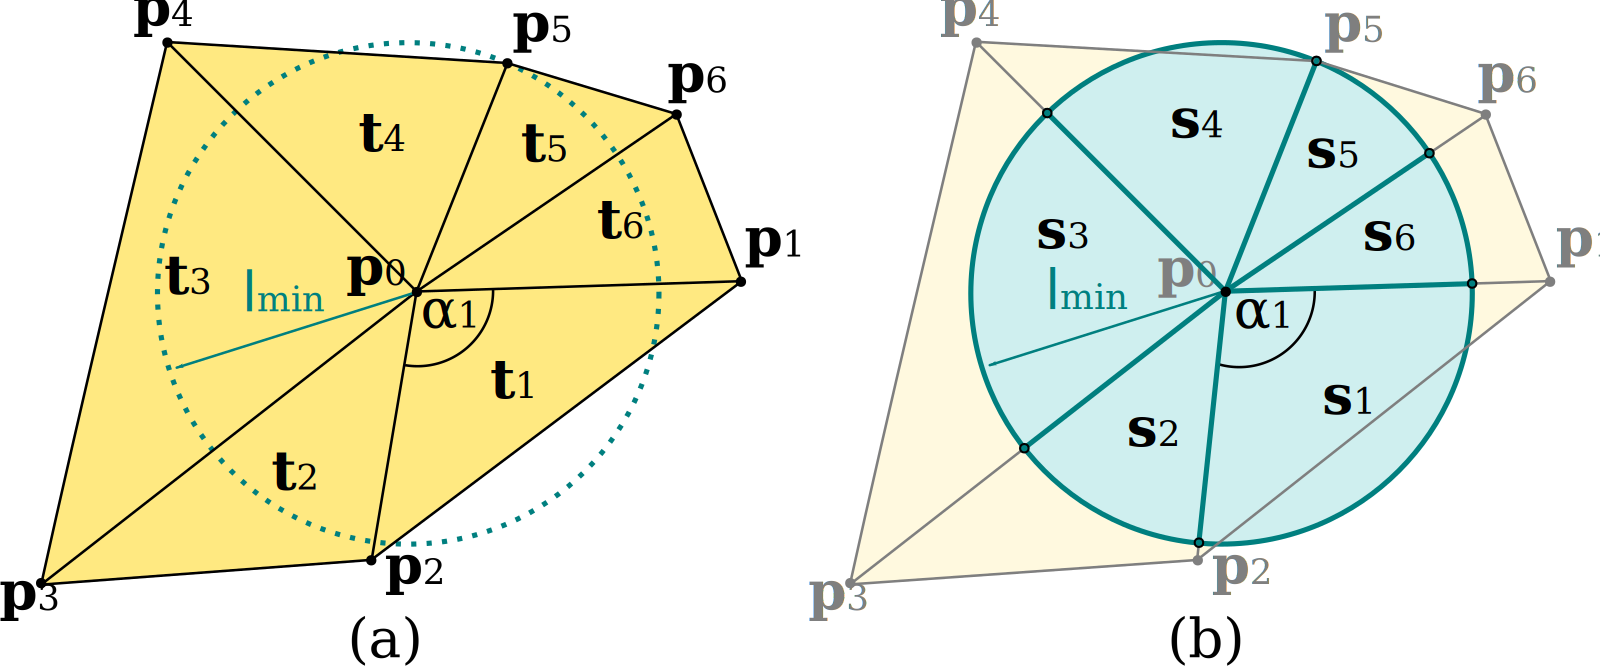
\includegraphics[width=1.0\linewidth]{figures/geodesicDisc.png}}
	{\caption[One-ring and geodesic disc]{A typical configuration of one-ring neighborhood $\bN_v$, described by (a) the six irregular triangular faces $\bt_i$ in sand color, which are defined by the six neighboring points $\bp_i$, which are all adjacent to the center point $\bp_0$; the smallest edge length $\elm = \elm(\bp_5) = |\bp_5 - \bp_0|$ illustrated with a teal arrow as the radius of the geodesic disc $\bO_v$, drawn as a dotted circle, also in teal color; and $\alpha_1$ as the central angle of $\bt_1$ (b) the complete geodesic disc $\bO$ composed of all six of the circular sectors $\bs_i$ which it circumscribes.}\label{fig:geodesicDisc}}
\end{figure}%

Furthermore, to ensure that the filter window size remains static for the duration of each convolution\todoResearch{call to question the importance of global minimum edge length in light of the typo found in source}, we define the global minimum edge length as
%
\begin{equation}
	\gelm := \min\left \{\elm(\bp_0) \;|\; \bp_0 \in \bM\,\right \}
	\label{eq:globalMinimumEdgeLength}
\end{equation}%
\nomenclature[jc]{$\gelm$}{the shortest edge length in $\bM$}%
%
and then use $\gelm$, the shortest edge length between any pair of adjacent points in the triangle mesh $\bM$, in lieu of the local minimum edge length $\elm(\bp_i)$, as the radius of the geodesic disc for all neighborhoods in all the following equations presented in this chapter.

%
%
%
\section{Interior Angles}
\label{ch4sIA}
Having now determined in the previous section, the global minimum edge length $\gelm$, we may now consider the next step in calculating \Fors{t}. Because we intend to use the area of each circle sector $\bs_i$ comprising the geodesic disc $\bO_v$ as weights upon the scalar field for averaging the function values per sector and per neighborhood, we must first calculate the inner angles $\alpha_i$ of each triangular face $\bt_i$ in the neighborhood $\bN_v$, for use in those later computations. These inner angles may be obtained by applying the Law of Cosines~\cite{Weisstein19e}
%
\begin{equation}
	\alpha_i = cos^{-1}(\frac{|\bp_0 - \bp_{i}|^2 + |\bp_0 - \bp_{\sipo}|^2 - |\bp_i - \bp_{\sipo}|^2}{2\cdot|\bp_0 - \bp_{i}|\cdot|\bp_0 - \bp_{\sipo}|})
\end{equation}
%
or more compactly:
%
\begin{equation}
	\alpha = cos^{-1}\left (\frac{\ell_c^2 + \ell_b^2 - \ell_a^2}{2\cdot\ell_c\cdot\ell_b}\right )
	\label{eq:alphaFromEdgeLengths}
\end{equation}%
\nomenclature[ka]{$\alpha$}{the central angle of circle sector $\bs_i$}%

 the function values . For those computations, we will require the value of the other inner angles $\beta_i$, which may be obtained by applying the

Also, it is our intention to interpolate and extrapolate the function values in relation to the distances between them and each of their adjacent points, thus we will be required to interpolate the values one side of the sector bisecting line at a time, as will be discussed in detail in Section~\ref{ch4sWM}. Having now obtained the first inner angles $\alpha_i$, we can now calculate the other inner angles $\beta_i$ using a proxy right triangle and the third angle theorem\footnote{otherwise known as the Angle-Angle-Angle Theorem, abbreviated as AAA}~\cite{Weisstein19f} as
%
\begin{equation}
	\beta = \Big(\frac{\pi}{2} - \frac{\alpha}{2}\Big) = \frac{(\pi - \alpha)}{2}
	\label{eq:betaFromHalfAlpha}
\end{equation}%
\nomenclature[kb]{$\beta$}{the third angle with $\frac{\alpha}{2}$ and $\frac{\pi}{2}$}%

Figure~\ref{fig:anglesAndCenterOfGravity} extends Figure~\ref{fig:geodesicDisc} by enhancing the circle sector $\bs_1$ to show an example of the angles $\alpha/2$ and $\beta$, with the proxy right triangles used to calculate it, as well as the center of gravity which is discussed in detail in Section~\ref{ch4sIACG}.

%
%
%
%
\section{Area \& Center of Gravity}
\label{ch4sIACG}
Because a circle sector may be described entirely by its radius and central angle~\cite{Weisstein19d}, having now calculated $\gelm$ and $\alpha$, the area of the sector can be obtained using the formula
%
\begin{equation}
	A = \frac{(\gelm)^2\alpha}{2}
	\label{eq:circularSectorArea}
\end{equation}
%
and similarly $\check{\ell}$, the distance from the center point $\bp_0$ along the bisecting line to the center of gravity $\bc$ can be calculated directly using the formula
%
\begin{equation}
	\check{\ell} := \frac{4\:\gelm\:\sin(\frac{\alpha}{2})}{3\,\alpha}
	\label{eq:distToCoG}
\end{equation}%

Figure~\ref{fig:anglesAndCenterOfGravity} extends Figure~\ref{fig:geodesicDisc} by enhancing the circle sector $\bs_1$ to illustrate the center of gravity $\bc$ and its distance from the center point $\bp_0$. In general, while holding the radius constant, the smaller the angle $\alpha$ becomes, the longer the distance $\check{\ell}$ becomes.

\begin{figure}[ht]
\ffigbox
	{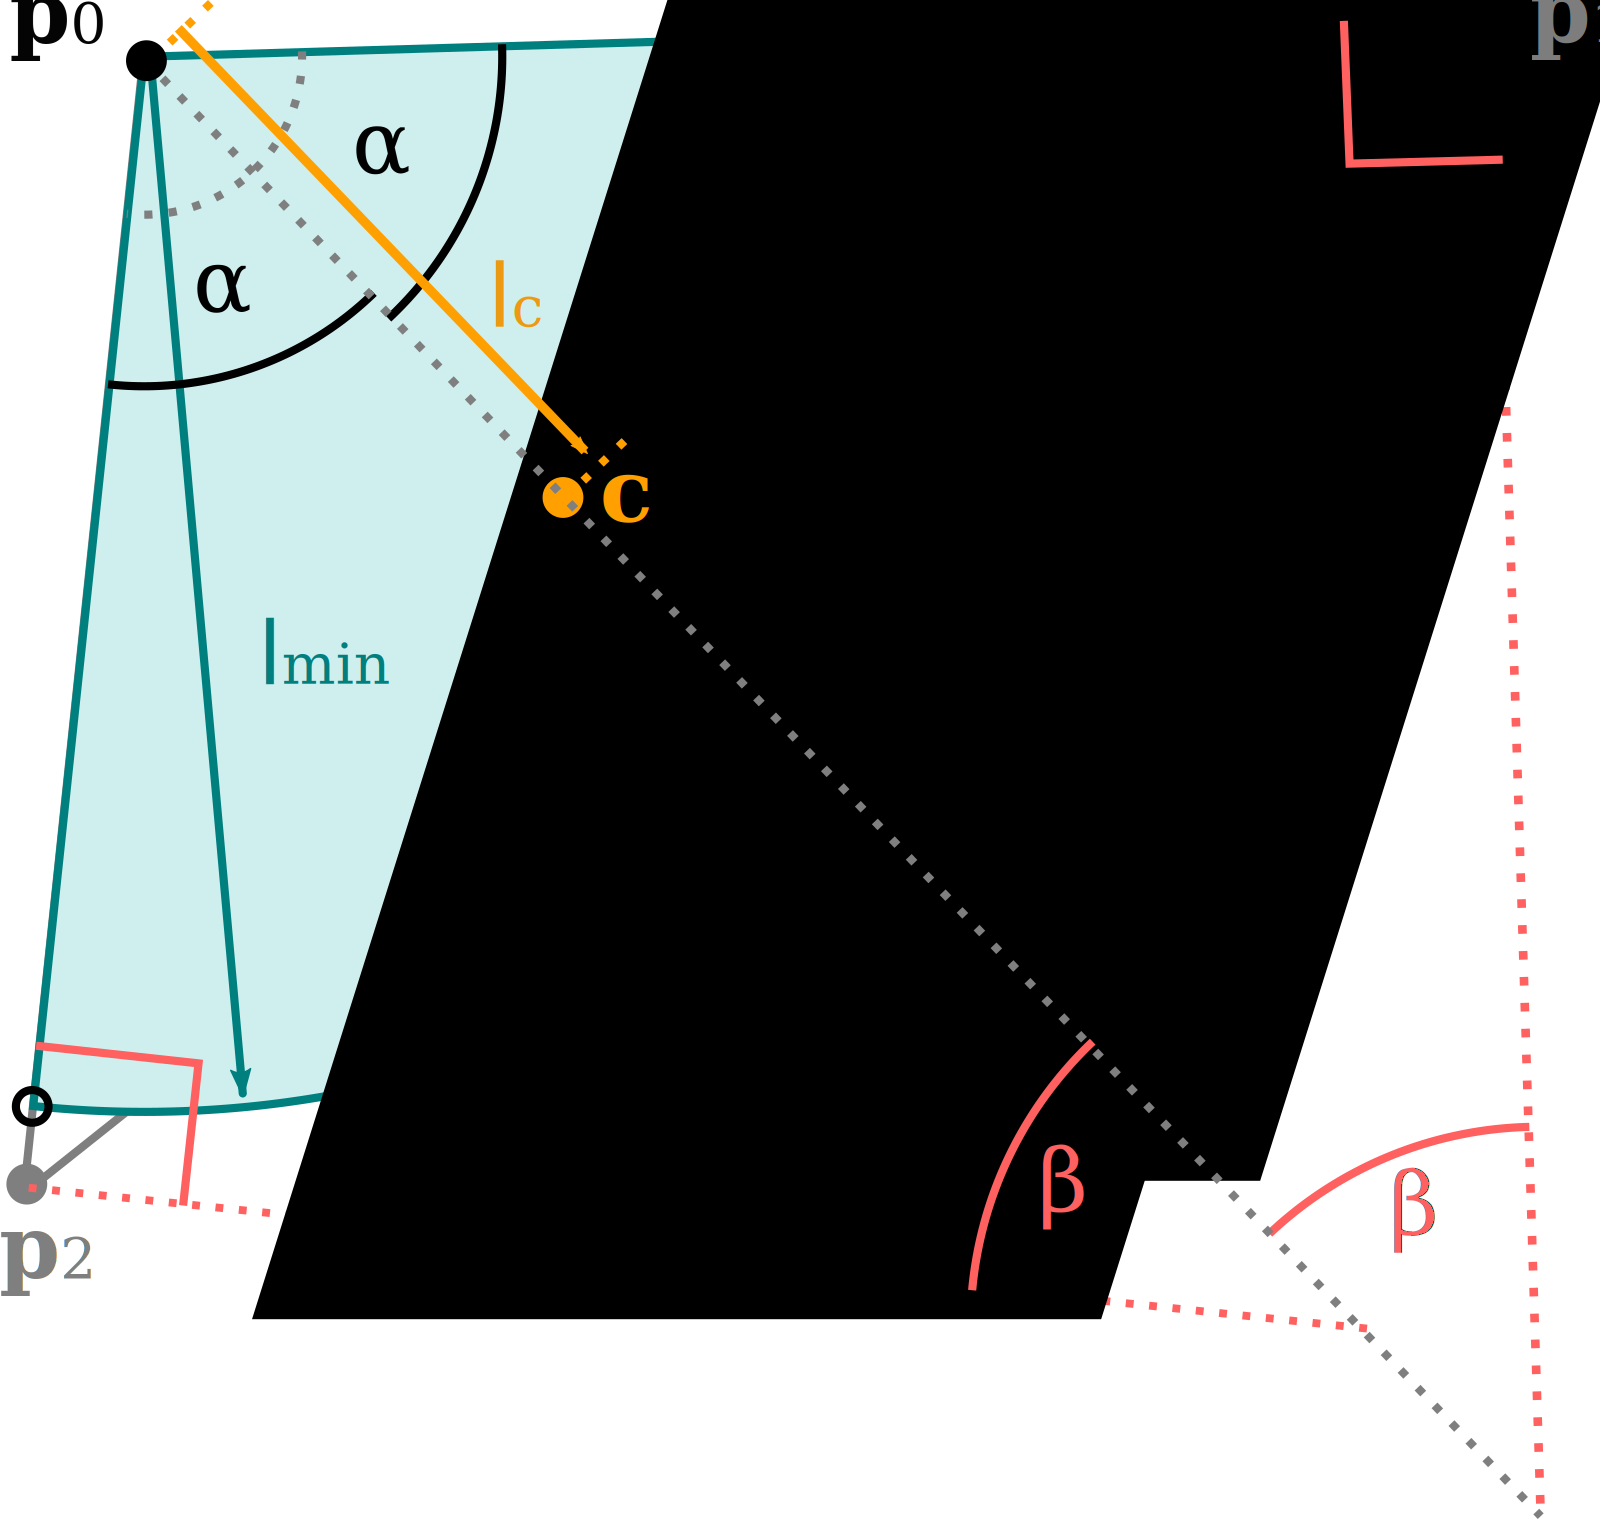
\includegraphics[width=0.8\linewidth]{figures/anglesAndCenterOfGravity.png}}
	{\caption[Angles and Center of Gravity]{An enhanced view of Figure~\ref{fig:geodesicDisc}, focusing on the circle sector $\bs_1$, showing $\alpha$ and the bisecting line in gray dots. In sand color is the center of gravity $\bc$ and $\check{\ell}$, the distance to it from $\bp_0$ along the bisecting line. Also shown in coral color, are the angles $\beta$, with the proxy right triangles used to calculate them.}\label{fig:anglesAndCenterOfGravity}}
\end{figure}%

%
%
%
%
\section{Interpolation \& Extrapolation}
\label{ch4sIE}
Given the scalar field\footnote{\fors{T} is agnostic to the meaning of information represented by the data stored as function values in scalar fields, therefore, it can similarly convolve any such data. However, because the filter was designed to only convolve scalar fields, any multi-dimensional data, such as RGB color, must be processed individually as independent scalar fields.} of function values $\bF$, and having now calculated $\beta$, and $\gelm$, both values which are constant between the two halves of the circle sector, we can next use the Law of Sines~\cite{Weisstein19g} to obtain the pairwise constant ratio
%
\begin{equation}
	\zeta = \frac{\gelm}{\sin(\beta)}
	\label{eq:zeta}
\end{equation}%
\nomenclature[la]{$\zeta$}{pairwise constant ratio for interpolation derived from Law of Sines}%

It should be noted, that because the points $\bp_j$ and $\bp_{\sjpo}$ are likely\footnote{One need only to look at Figures~\ref{fig:geodesicDisc} or~\ref{fig:anglesAndCenterOfGravity} for an example of why that may be.} at different distances from the center point $\bp_0$, we must now begin calculating for each half of the circular sector individually. Therefore, while the index for $\zeta$ remains the match for the index of the circle sector $\bs$, we will now use the index $j$ to denote the side of the sector defined by its point $\bp_j$ or $\bp_{\sjpo}$.

Next, using $\zeta$, we can interpolate the offset from the original function values $f_j$ and $f_{\sjpo}$ at the points $\bp_j$ and $\bp_{\sjpo}$.
\begin{align}
	\tilde{\ell}_j & = \kern2pt\frac{\zeta}{\kern2pt\ell_j\kern2pt}\kern1pt = \kern3pt\frac{\zeta}{|\bp_j - \bp_0|}
	\label{eq:distanceIForInterpolation}\\
	\tilde{\ell}_{\sjpo} & = \frac{\zeta}{\ell_{\sjpo}} = \frac{\zeta}{|\bp_{\sjpo} - \bp_0|}
	\label{eq:distanceIp1ForInterpolation}
\end{align}%
\nomenclature[lb]{$\tilde{\ell}_j$}{also $\tilde{\ell}_{\sjpo}$, the distances for interpolation of $f_j$ and of $f_{\sjpo}$ towards $f_0$}%

Then, applying the offset distances $\tilde{\ell}_j$ and $\tilde{\ell}_{\sjpo}$, to the original function values $f_0$, $f_j$, and $f_{\sjpo}$, we can now interpolate the function values at $\bp_j$ and $\bp_{\sjpo}$ as
\begin{align}
	f'_j & = f_0\,(1 - \tilde{\ell}_j) + f_j\,\tilde{\ell}_j
	\label{eq:interpolatedFi} \\
	f'_{\sjpo} & = f_0\,(1 - \tilde{\ell}_{\sjpo}) + f_{\sjpo}\tilde{\ell}_{\sjpo}
	\label{eq:interpolatedFip1}
\end{align}%
\nomenclature[lc]{$f'_j$}{also $f'_{\sjpo}$, the interpolated values of $f_j$ and $f_{\sjpo}$ toward $f_0$}%
\todoStyle{should I be using the $\bff$ macro?}

Figure~\ref{fig:interpolatedFunctionValues} illustrates an enhanced view of the circle sector $\bs_1$, continuing with the example introduced in Figure~\ref{fig:geodesicDisc}. It shows how, as a result of \tdd{} being composed of a discrete manifold, therefore, all function values must be stored 1-for-1 at the location of each point, instead of simply interpolating the function values at the corners of the geodesic disc, which are at the distance $\gelm$ between $\bp_0$ and $\bp_j$ or $\bp_{\sjpo}$, we must\todoAsk{but must we? we aren't ever going to save these values since they are unique to every neighborhood} instead interpolate as if $f_j$ were at $\gelm$, then calculate the $f'_j$ at the point $\bp_j$, so that either $f_0 \leq f_j \leq f'_j$ or $f_0 \geq f_j \geq f'_j$ are true\footnote{or both in the case that $\ell_j$ is equal to $\gelm$}, then likewise for $f'_{\sjpo}$. Furthermore, it illustrates how we must also interpolate from the points to the center of gravity, which we will discuss in detail Section~\ref{ch4sWM}.
\todoReword{update after change to fig}

\begin{figure}[ht]
\ffigbox
	{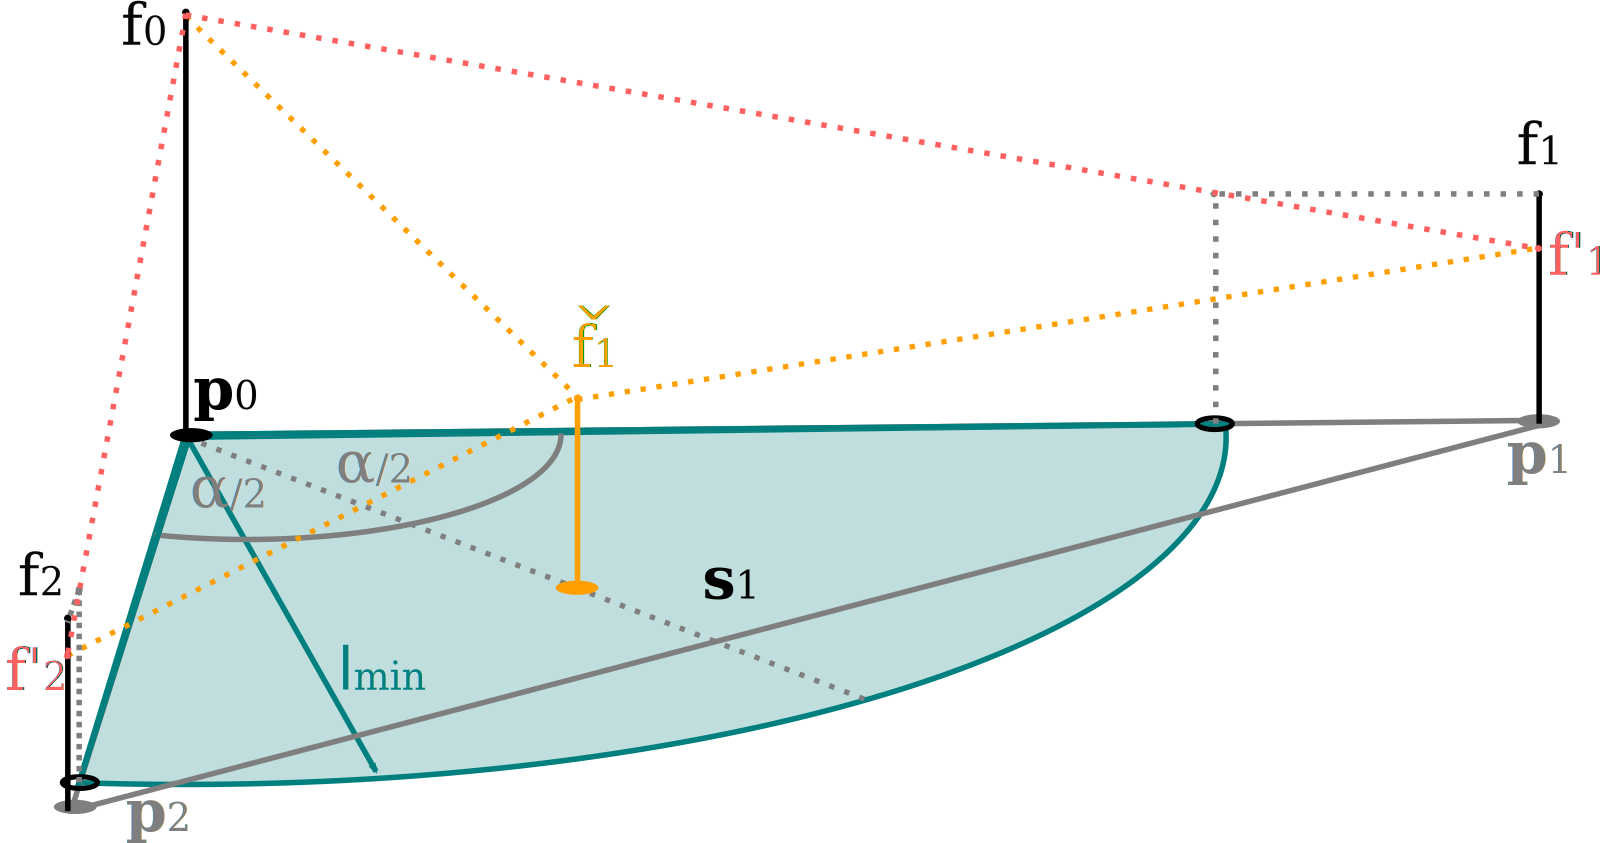
\includegraphics[width=1.0\linewidth]{figures/interpolatedFunctionValues}}
	{\caption[Interpolation of Function Values toward the Center of Gravity]{An enhanced view of the circle sector $\bs_1$, continuing with the example introduced in Figure~\ref{fig:geodesicDisc}, labeled in black are the function values $f_0$, $f_1$, and $f_2$, with the height of the line indicating magnitude of the value. Drawn in coral color, are the interpolated function values $f'_1$ and $f'_2$, along with the dotted lines illustrating how they were determined. In sand color is $\check{f}_1$, the weighted mean function value for the entire sector.}\label{fig:interpolatedFunctionValues}}
\end{figure}
\todoReword{after update to figure}

%
%
%
%
\section{Weighted Mean}
\label{ch4sWM}
In order to calculate the weighted mean function value at the center of gravity $\bc$, of the circle sector $\bs_i$, we must combine the original function value at the center point $f_0$, and both interpolated function values, $f'_j$ and $f'_{\sjpo}$. Then using the distance to the center of gravity $\check{\ell}$, and the formula
\begin{equation}
	\check{f} = f_0\,(1 - \check{\ell}) + \frac{(f'_j + f'_{\sjpo})\,\check{\ell}}{2}
	\label{eq:weightedMeanAtCoGatSector}
\end{equation}%
\nomenclature[ma]{$\check{f}$}{the weighted mean function value at $\bc$ of $\bs_i$}%
we obtain the weighted mean function value $\check{f}$, at the center of gravity, representing the entire circle sector.

Figure~\ref{fig:interpolatedFunctionValues} illustrates $\check{f}_1$ in sand color as a volume over an enhanced view of the circle sector $\bs_1$, continuing with the example introduced in Figure~\ref{fig:geodesicDisc}. The figure also shows details pertaining to the interpolation of the function values $f_j$ and $f_{\sjpo}$, as discussed in detail in Section~\ref{ch4sI}.
\todoReword{update after changes to figure}


Finally, we can multiply each interpolated function value located at each circle sector's center of gravity $\check{f}_i$, by each sector's area $A_i$, to obtain a volume of function value over the entire circle sector. Then by dividing the sum of all those sector-wise function value volumes by the total area of the geodesic disc $\bO_v$, we can compute
\begin{equation}
	f'_v := \frac{\sum A_i\check{f}_i}{\sum A_i} \quad \forall i \in \{1,\ldots,\,|\bN_v|\}
	\label{eq:meanFuncValAtPv}
\end{equation}%
\nomenclature[mb]{$f'_v$}{the one-ring weighted mean function value at $\bp_v$}%
the one-ring weighted mean\footnote{\fors{T} can be modified to use the median operation, instead of the mean, by using all the equations except Equation~\ref{eq:meanFuncValAtP0} and then sorting the results of Equation~\ref{eq:weightedMeanAtCoGatSector}. The details of which can be found by the original publication ~\cite[s.~3.2]{Mara17}, but as it was not implemented in GPGPU for this thesis, we exclude the details here.} function value for $\bp_v$, which is the center point $\bp_0$ of the neighborhood $\bN_v$.

Figure~\ref{fig:funcValVolumes} illustrates the geodesic disc $\bO$, as introduced in Figure~\ref{fig:geodesicDisc}, with volumes of interpolated function value over each circle sector, which shall be divided by each sector's area in order to obtain the the one-ring weighted mean function value $f'_v$ at $\bp_v$.
\begin{figure}[ht]
\ffigbox
	{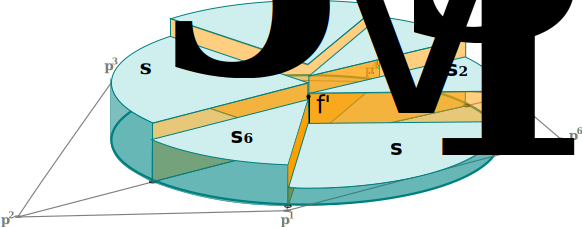
\includegraphics[width=1.0\linewidth]{figures/funcValVolumes.png}}
	{\caption[Weighted Mean Function Value $f'_v$at $\bp_v$]{The geodesic disc $\bO$, as introduced in Figure~\ref{fig:geodesicDisc}, with volumes of interpolated function values over each circle sector $\bs_i$, which shall be divided by each sector's area $A$ in order to obtain the the one-ring weighted mean function value $f'_v$ at $\bp_v$.}\label{fig:funcValVolumes}}
\end{figure}

As with any smoothing filter, there is no upper limit to the count of iterations one can convolve, however, the function values will all eventually converge at the global mean average function value. More details can be found in Section~\ref{ch3s2}.\todoCitation{mara on iteration count vs filter size}.\todoReword{elaborate}

%
%
%
\section{Summary}
\label{ch4sS}
In this chapter we presented an updated version of \Fors{t}, which since its original publication~\cite[s.~3.2]{Mara17}, now utilizes the entire area of each sector $\bs$ of the geodesic disc $\bO$ centered at each point $\bp_v$ in the mesh $\bM$, in order to calculate the weighted average of all the function values in its one-ring neighborhood. First, we illustrated in detail how one can calculate the globally shortest edge length $\gelm$, interior angles $\alpha$ and $\beta$, the area $A$, and the distance $\check{\ell}$ from the center point to the center of gravity $\bc$, for any given of circle sector in a one-ring neighborhood $\bN$. Next, we provided the equations for interpolating the three function values $f_0$, $f_j$, and $f_{\sjpo}$, using the pairwise constant ratio $\zeta$ in order to obtain the weighted mean function value $\tilde{f}$ for each $\bs$, and finally the weighted mean function value $f'_v$ at point $\bp_v$, representing the entire one-ring neighborhood $\bN$. Convolving this filter at each vertex in the mesh, with the scalar field of function values $\bF$, for any number of iterations, thus produces a smoothing effect with increasing intensity in relation to the number of iterations.
